%------------------------------------------------------------
% Description : Differential Geometry
% Author      : Iliya Tikhonenko <iliya.t@mail.ru>
% Created at  : Thu Jun  1 18:33:27 MSK 2017
%------------------------------------------------------------
\documentclass[draft,timbord]{longnotes}
\usepackage{tmath} 
\usepackage{cussymb} 
\usepackage{silence}
\WarningFilter{latex}{Reference}
\graphicspath{{../../img/}}
\begin{document}

\paragraph{Регулярная кривая и её естественная параметризация}
\label{par:dg::curve}

\begin{defn}[Кривая, как отображение]\label{defn:dg::curve::map}
  Пусть задано гладкое отображение $t\in [a;b] \mapsto r(t) \in \R^3$, регулярное, то есть
  $\rk r'(t) \equiv 1$. $t$~--- параметр, само отображение ещё можно
  называть параметризацией.

\end{defn}

\begin{defn}[Кривая, как класс отображений]\label{defn:dg::curve::class}
  Введём отношение эквивалентности отображений:
  \[
    r(t) \sim \rho(\tau) \Leftrightarrow 
    \exists\, \delta \colon [a;b] \leftrightarrow [\alpha, \beta ] \that \rho (\delta (t)) = r(t)
  \]
\end{defn}

А теперь будем их путать. \flame
Ещё веселье с многообразиями.

\begin{defn}[Естественная параметризация]\label{defn:dg::curve::nat}
  Пусть $[a;b] = [t_0, t_1]$.
  Рассмотрим $\ov~s(t) = \dint_{t_0}^t | r'(t) | \, \del \tau $. Она, как видно, является 
  пройденным путём и неубывает  $ \Rightarrow $ годится на роль $\delta$.

  Так что можно рассматривать $s$ как параметр,  это собственно и есть
  естественная (натуральная) параметризация.
\end{defn}


\begin{prop}\label{prop:dg::curve::repar}
  Пусть есть две разных параметризации: $r(t)$ и $r(s)$ одной кривой. Тогда 
  \[
    \dot r \equiv \pder{r(s)}{s} = \Bigl(r'(t) \cdot (s'(t))^{-1}\Bigr)(t) = \frac{r'}{|r'|} 
  \]
  Как видно, натуральная почему-то обозначается точкой.
\end{prop}

\paragraph{Кривизна кривой}
\label{par:dg::curvature}

\begin{defn}[Касатальный вектор]\label{defn:dg::curvature::tang}
  $\tau := \dot r(s)$.
\end{defn}

\begin{defn}[Кривизна]\label{defn:dg::curvature}
  $k_1 = |\dot \tau |$
\end{defn}
\begin{defn}[Радиус кривизны]\label{defn:dg::curvature::rad}
  $R = k_1 ^{-1}$
\end{defn}

\begin{lem}\label{lem:dg::curvature::fixnorm}
  Пусть $v (s) \in \R^n$, $|v| \equiv R \in \R$.
 Тогда $\dot v \perp v$.
\end{lem}
\begin{lproof}
  $0 = \fder{}{t}\, {|v|^2} = \fder{}{t}\,  (\langle v,v \rangle) = 2 \langle v,\dot v \rangle$.
  Так что $\langle v \dot v \rangle = 0 \Rightarrow v\perp \dot v $.
\end{lproof}

\begin{prop}\label{prop:dg::curvature::orth}
  $\tau \perp \dot \tau$
\end{prop}


\begin{thrm}\label{thrm:dg::curvature::repar}
  Пусть $r(t)$~--- неестественная параметризация кривой. Тогда
  $\displaystyle k_1 = \frac{| r' \times r''|}{|r'|^3} $
\end{thrm}

\begin{tproof}
  \begin{align*}
    k_1 &= |\dot \tau | = \left| \fder{}{s}\, \frac{r'}{|r'|} \right| 
    =\left| \fder{}{t} \left(\frac{r'}{|r'|}\right) \, \fder{t}{s}  \right|
    =\left| \fder{}{t} \left(\frac{r'}{|r'|}\right) \, \frac{1}{|r'|}  \right| \\
    \fder{}{t} \left(\frac{r'}{|r'|}\right) &=  \frac{r'' |r'| - r' |r'|'}{|r'|^2} , 
    \quad |r'|' = \left(\sqrt{r'^2}\right)' = \frac{\langle r', r'' \rangle}{|r'|} \\
    \fder{}{t} \left(\frac{r'}{|r'|}\right) &=  \frac{r'' |r'|^2 - r'\langle r', r''\rangle}{|r'|^3}
    =  \frac{r'' \langle r', r' \rangle  - r'\langle r', r''\rangle}{|r'|^3}
    =  \frac{r' \times (r'' \times r') }{|r'|^3} \; (A=C)\\
    \intertext{ $r' \perp r' \times r''$, так что} \\
    k_1 &= \left| \frac{r' \times (r'' \times r') }{|r'|^3} \right| \, \frac{1}{|r'|}
    = \frac{|r' \times r''|}{|r'|^3} 
  \end{align*}
\end{tproof}

\paragraph{Кручение и нормаль}
\label{par:dg::norm}

\begin{defn}[Нормаль]\label{defn:dg::norm::norm}
  Пусть $k_1 \neq 0$. Тогда $\nu  := \frac{\dot \tau } {k_1}$.
\end{defn}
из геометрии, она лежит в плоскости кривой и направлена в сторону <<поворота>>. 
\begin{defn}[Бинормаль]\label{defn:dg::norm::binorm}
  $\beta = \tau \times \nu $.
\end{defn}

\begin{rem*}
  $(\tau,\nu,\beta)$~--- хороший кандидат для репера в какой-нибудь точке $P$.
\end{rem*}
\begin{defn}[Соприкасающаяся плоскость]\label{defn:dg::norm::tangpl}
  Пусть $k_1 > 0$, $P = r(s_0)$, $T$~--- плоскость, $T \ni P$, $N \perp T$~--- нормаль к ней.
  Допустим, $ \langle \Delta r, N \rangle = h$, $h = o(\Delta s^2)$. Тогда $T$~--- соприкасающаяся
  плоскость.
\end{defn}
\begin{prop}\label{prop:dg::norm::tangpl}
  $ \tau , \nu \perp N  $;
  $(r-r_0, \dot r_0 , \ddot r_0)=0$~--- её уравнение
\end{prop}
\begin{lproof}
  \[
    \begin{split}
      \Delta r = \dot r  \, \del s + \frac{\ddot r}{2} \, \del s^2 + o(\Delta s^2)
      &= \tau \, \del s + \frac{1}{2} \, k_1 \nu \, \del s^2 + o(s^2) \\
      &\langle \Delta r , N \rangle = o(\Delta s^2) 
    \end{split}
  \]
  Так что скалярные произведения $\langle \tau,  N\rangle$, $\langle \nu,  N\rangle$ равны нулю.
  
  Вторая часть~--- из свойств смешанного произведения.
\end{lproof}

\begin{defn}[Абсолютное кручение]\label{defn:dg::norm::abscrvn}
  $|k_2| := | \dot\beta|$
\end{defn}
\begin{thrm}\label{thrm:dg::norm::abscrvn}
  $|k_2| = \left|\dfrac{(\dot r, \ddot r, \dddot r\,)}{k_1^2}\right|$
\end{thrm}

\begin{tproof}
  Взять определение $\beta$ и посчитать производную.
  \[
    \dot \beta  = \dot \tau \times \nu + \tau \times \dot \nu 
    = k_1 \nu \times \nu + \tau \times \dot \nu  = \tau \times \dot \nu 
  \]

  Производная $\tau$ ничем не отличается от \ref{thrm:dg::curvature::repar}, 
  только $\tau$ заместо $r$.
  
  Так что
  \[
    \dot \beta = \tau\times(\dot \tau \times(\ddot\tau \times \dot\tau))\,\frac{1}{k_1^3}
    = \frac{\dot\tau (\tau, \ddot \tau , \dot \tau) -(\ddot\tau \times \dot\tau)\cdot 0 }{k_1^3} 
    = -\frac{\nu \cdot (\tau, \dot \tau , \ddot \tau)  }{k_1^2} 
  \]
\end{tproof}

\begin{defn}[Кручение]\label{defn:dg::norm::crvn}
  $k_2 := \dfrac{-(\dot r, \ddot r, \dddot r\,)}{k_1^2}$
\end{defn}

\paragraph{Формулы Френе}
\label{par:dg::frene}

\begin{thrm}\label{thrm:dg::frene}
  \begin{equation}
    \label{eq:dg::frene}
    \begin{pmatrix}
      \dot\tau \\\dot\nu \\ \dot\beta
    \end{pmatrix}
    = 
    \begin{pmatrix}
      0 & k_1 & 0 \\
      -k_1 & 0 & -k_2 \\
      0 & k_2 & 0
    \end{pmatrix}\cdot
    \begin{pmatrix}
      \tau \\ \nu \\ \beta
    \end{pmatrix}
  \end{equation}
\end{thrm}

\begin{tproof}
  Осталось доказать лишь второе, но оно очевидно следует из 1 и 3 и соотношения 
  $\nu = \beta \times \tau$.
\end{tproof}

\begin{thrm}\label{thrm:dg::frene::reconst}
  Пусть $r(s)$~--- гладкая кривая с заданными $k_1$ и $k_2$, $k_1>0$. 
  Тогда система \eqref{eq:dg::frene} определит её с точностью до движения.
\end{thrm}

\begin{tproof}
  Система \eqref{eq:dg::frene} вообще линейна. Так что решение задачи Коши у неё~--- единственно.
  А положение кривой как раз задается начальными значениями $\tau , \nu , \beta $.

  Давайте покажем, что полученные векторы~--- ортонормированный базис.
  \begin{align*}
    \fder{}{t}(|\tau|^2)  &= 2 k_1 \langle \tau, \nu \rangle \\
    \fder{}{t} (|\nu|^2)  &= -2 k_1 \langle \nu, \tau \rangle - 2 k_2 \langle \nu , \beta \rangle\\
    \fder{}{t} (|\beta|^2)  &= 2 k_2 \langle \beta, \tau \rangle \\
    \fder{}{t} (\langle \tau, \nu \rangle)  
    &= k_1 |\nu|^2 - k_1 |\tau|^2 - k_2 \langle \beta, \tau \rangle \\
    \fder{}{t} (\langle \nu, \beta \rangle)  
    &= -k_2 |\beta|^2 + k_2 |\nu|^2 - k_1 \langle \tau,\beta \rangle \\
    \fder{}{t} (\langle \beta,\tau \rangle)  
    &= k_2 \langle \nu, \tau \rangle + k_1 \langle \beta, \nu  \rangle
  \end{align*}
  Получилась очень большая линейная система. Решение, когда все векторы ортогональны и единичны
  нас вполне устроит. Так что, если при $s=0$ условие ортонормированности выполнено, то оно
  выполено и во все моменты времени.

  Правда ниоткуда не следует, что кривизна и кручение будет какими надо, но это
  из формул для них докажется.
\end{tproof}


\paragraph{Регулярная поверхность. Касательная плоскость. Первая квадратичная форма}
\label{par:dg::tangplane}

\begin{defn}[Поверзность (двумерная)]\label{defn:dg::tangplane::manifold}
  Пусть задано гладкое отображение \[
    \varphi \colon (u,v) \in D \subset \R^2 \mapsto r=(x,y,z) \in \R^3
  \]
  Добавим условие регулярности $\rk \varphi' \equiv 2$ и условимся путать отображение и класс 
  оных.
\end{defn}

\begin{defn}\label{defn:dg::tangplane::tanv}
  \[
    \begin{split}
      r_u &:= (x_u', y_u', z_u') \\
      r_v &:= (x_v', y_v', z_v') \\
      n &:= \frac{r_u \times r_v}{|r_u \times r_v|} = \frac{N}{|N|} 
    \end{split}
  \]
  Отметим, что условие регулярности не дает векторному произведению обращаться в 0.
  
  Касательную плоскость можно было бы здесь определить через нормаль, но лучше пока ещё подумать.
  Может, абстракций добавить.
\end{defn}

Просто утащил определеньки из \ref{par:dg::orient}
\def\H{\mathbbm H}
\begin{defn}\label{defn:dg::manifold}
  Пусть $M \subset \R^n$. Выберем на нем произвольную точку $x$ и рассмотрим 
  $V(x) = V_{\R^n}(x) \cap M$. Допустим, 
  \[
    \exists\, f \in C^1 \that V(x) \leftrightarrow^f \R^k\;(\text{или }\H^k).
  \]
  
  Тогда $M$~--- гладкое подмногообразие $\R^n$, а $f$~--- локальная карта многообразия.
  Набор всех карт называется атласом. $t \in \R^k$~--- локальные координаты в $V$.
  
  Атлас : $A(M) = \{(\varphi_k, V_k)_k\}$~--- все окрестности и карты на них. 

  Если 
  \[
    \exists\, x\in M \that V \leftrightarrow \H (\H = \{x\in \R^k \mid x^1 \leqslant 1\},
    \] 
  тогда это многообразие с краем.  
  Край обычно обозначается как $\partial M$.

  По идее, в атлас ещё надо включать информацию, карта на $\R^k$ или на $\H^k$. Так что
  \[
    A(M) = \{ (\H^k, \varphi_i, V_i)_i\} \cup \{(\R^k, \varphi_j, V_j)_j\}
  \]
\end{defn}
\begin{defn}[Касательное пространство в точке $x$]\label{defn:dg::tangentbndl}
  Пусть $M$~--- гладкое многообразие. Допустим, $\varphi_i$~--- карта в $V(x)$.
  Тогда
  \[
    T_x M = \Bigl(\del \varphi_i (x)\Bigr)(\R^k) 
  \]
\end{defn}

Так что разумнее рассматривать повехность, как двумерное многообразие. 


\begin{defn}[Первая квадратичная форма]\label{defn:dg::tangplane::I}
  \[
    \begin{split}
      I :&= |\del r|^2  = r_u^2\, \del u^2 + 2r_u r_v\, \del u \,\del v + r_v^2\, \del v^2 \\
        &= E \, \del u^2 + 2F\, \del u \,\del v + G\, \del v^2 
    \end{split}
  \]
\end{defn}
Плохое определение, надо сказать. Сделаем получше.

\begin{defn}\label{defn:dg::tangentbndl::Ibetter}
  Первая квадратичная форма поверхности $M$~--- единичная 
  квадратичная форма на его касательном пространстве. 
\end{defn}

Скаляряное произведение на $T_x M$ можно перенести из $\R^m \supset M$. 

\begin{prop}\label{prop:dg::tangentbndl::Ipar}
  Пусть $\varphi \colon D \subset M$~--- карта на $M$. Тогда первая квадратичная форма в 
  координатах пространства параметров имеет вид 
  \[
    L^T L , \quad L = \varphi'(x)
  \]
\end{prop}

Мы вроде можем спокойно рассматривать $\varphi'$ как линейное отображение.
Так что по идее первое определение~--- следствие отсюда, но \quest.

\begin{defn}\label{defn:dg::tangentbndl::gram}
  $g_{ij} = L^T L$. Хотелось бы сказать, что это метрический тензор, но не стоит.
\end{defn}

\paragraph{Вычисление длин и площадей на поверхности}
\label{par:dg::area}

\begin{thrm}\label{thrm:dg::area::len}
  Пусть $M$~--- поверхность, $\gamma \colon t \to r \in M$.
  Тогда \[
    \ell(\gamma)= \dint_{t_0}^{t_1} \sqrt I.\; (\del s = I)
  \]
\end{thrm}
\begin{tproof}
  Пусть $r \in M$, $u \in D$. Тогда
  $\del s^2 = \langle \del r, \del r \rangle = \del r ^T \del r = \del u^T L^T L \del u = I$.
  А дальше можно параметризовать кривую, так что $u,v$~--- функции от $t$. 
\end{tproof}


Некое пояснение к определению.

Здесь можно сказать, что  мера на касательном многообразии
задаётся как образ лебеговой меры в $\R^k$.
Они вроде как имеют одну размерность.
Правда его надо как-то повернуть для этого, иначе якобиан не посчитать.

Зафиксируем какие-то базисы в $D$ и $T_xM$.
Соорудим вот такое ортогональное преобразование: $O = \left(\sqrt{I}\right)^{-1} L^T$,
$O \colon \R^m \to \R^m$, скалярное произведение в них одинаковое.

Здесь неявно сконструировали отображение $I\colon \R^k \to \R^k$ взяв матрицу $I$.

Тогда пусть $F = O \circ L = \left(\sqrt{I}\right)^{-1} L^T L = \sqrt{I}$.
Пользуясь теоремой из теории меры, $\lambda_T = \det F = \det \sqrt I = \sqrt {\det I}$.
Кажется, наш Франкенштейн создан.

А теперь можно приближать параллелепипеды на самом многообразии
похожими из касательного пространства.


\begin{defn}\label{thrm:dg::area::manifold}
  Пусть $M$~--- подмногообразие $\R^n$.  Тогда 
  \[
      \lambda_k := \int _D \sqrt {\det g(t)} \, \del t, \quad
      g(t)_{ij} = \left(\pder{x}{t_i} \cdot \pder{x}{t_j}\right)\, (t)
  \]
\end{defn}

\begin{thrm}\label{thrm:dg::area::manifoldcor}
  Определение выше не зависит от параметризации.
\end{thrm}

\begin{thrm}\label{thrm:dg::area::area}
  Пусть $M$~--- поверхность, $u,v\in D$, $I = E \, \del u^2 + 2F\, \del u \,\del v + G\, \del v^2$.
  Тогда
  \[
    S(M) = \iint_D \sqrt{EG - F^2}\, \del u\,\del v
  \]
\end{thrm}

\begin{defn}\label{defn:dg::area::isom}
  Пусть $M_1$, $M_2$~--- пара поверхностей. Допустим, $\exists\, F \colon M_1 \to M_2$, 
  сохраняющее длины кривых. Тогда они называются  изометричными.
\end{defn}

\begin{thrm}\label{thrm:dg::area::Iisom}
  Пусть $M_1$, $M_2$~--- пара поверхностей. Допустим, что существуют их параметризации, 
  при которых $I_1= I_2$. Тогда они изометричны.
\end{thrm}

\paragraph{Вторая квадратичная форма}
\label{par:dg::II}

\begin{defn}\label{defn:dg::II}
  Снова рассмотрим поверхность с  какой-то параметризацией. Тогда 
  ${\rm II} := - \del r \, \del n = L \, \del u^2 + 2N\, \del u \,\del v + M\, \del v^2$.
\end{defn}

Не совсем понятно, как определить нормаль в общем случае, но наверное
можно построить такой же определитель как и для векторного произведения.

\begin{prop}\label{prop:dg::II}
  ${\rm II} = n \cdot \del^2 r$
\end{prop}
\begin{lproof}
  Расписать.
\end{lproof}

\begin{prop}[Типы точек на поверхности]\label{prop:dg::II::ptypes}
  Здесь названия связаны с типом соприкасающегося параболоида. Его можно добыть, рассматривая
  $\langle \Delta r, n \rangle$.
  \[
    \langle \Delta r ,n \rangle = \underbrace{\langle \del r, n \rangle}_0
    + \frac{1}{2} \underbrace{\langle \del^2 r, n \rangle}_{\rm II} + 
    o(\del^2 r)
  \]
  \begin{description}
    \item[${\rm II} > 0$:] Эллиптический
    \item[${\rm II} < 0$:] Он же
    \item[${\rm II} \lessgtr 0$:] Гиперболический
    \item[${\rm II} \geqslant 0 \lor {\rm II} \leqslant 0$:] Параболический (вроде цилиндра)
    \item[${\rm II} = 0$:] Точка уплощения
  \end{description}
\end{prop}


\paragraph{Нормальная кривизна в данном направлении. Главные кривизны}
\label{par:meas::curfctr}

\begin{defn}\label{defn:meas::curfctr::normsec}
  Нормальное сечение поверхности~--- сечение плоскостью, 
  содержащей нормаль к поверхности (в точке).
\end{defn}

\begin{lem}\label{lem:meas::curfctr::normsec}
  Нормальное сечение~--- кривая.
\end{lem}

Сначала рассмотрим несколько более общий случай

\begin{thrm}[Менье]\label{thrm:meas::curfctr::menie}
  Пусть $\gamma$~--- кривая $ \subset M$, $ \gamma \ni P$.
  Тогда $k_0 = k_1 \cos (\underbrace{\nu \,\text{\^;}\, n}_\theta) = \frac{\rm II}{\rm I} $.
\end{thrm}
\begin{tproof}
  $\ddot r = \dot \tau = k_1 \nu $.
  Так что $\langle \ddot r, n \rangle =  k_1 \langle \nu, n \rangle$.
\end{tproof}

\begin{rem}\label{rem:meas::curfctr::menie::ref}
  Ещё можно сформулировать так: для всякой кривой на повехности, проходящей через точку 
  в заданном направлении $k_0 = \rm const$
\end{rem}

а теперь сузим обратно.
\begin{defn}\label{defn:meas::curfctr::normcrvf}
  Нормальная кривизна~--- кривизна нормального сечения.
\end{defn}

Для нормального сечения $\cos\theta = \pm 1$.

Если немного переписать и ввести параметр $t= \del v /\del u $
\[
  k_1(t) = |k_0(t)| = \left|\frac{L + 2Nt + Mt^2}{E + 2Ft +Gt^2} \right|
\]
Этот параметр $t$ и задаёт <<направление>> нормального сечения. 
Так что $k_0(t)$ и есть та самая <<кривизна в данном направлении>>.

Теперь найдем экстремумы $\frac{\rm II}{\rm I} (t)$. 
\begin{thrm}\label{thrm:meas::curfctr::minmax}
  $\exists\, k_{\min}, k_{\max}$, $k_{\min} \cdot k_{\max} = \frac{LM - N^2}{EG - F^2}$.
\end{thrm}
\begin{tproof}
  По теореме из линейной алгебры, пару квадратичных форм можно привести к диагональному виду.
  Это возможно, если одна из них неотрицательна, она выбирается за скалярное произведение.

  Хорошо, будем искать экстремумы той дроби для единичных векторов из касательного пространства. 
  Вектор единичный, если его скалярное произведение с самим собой единичное. А для 
  векторов из касательного пространства сама первая квадратичная форма единична.

  Короче, она уже будет приведена к диагональному виду во всех базисах $T_xM$. Ещё
  есть свобода вращать там векторы, воспользуемся ей. 

  Известно, что условный экстремум квадратичной формы~--- на собственных векторах. 
  Выберем их за базис. Он будет ортогональным, ведь форму привели к диагональному виду.

  Переходя в исходные координаты, получим утверждение теоремы.
\end{tproof}

\begin{defn}\label{defn:meas::curfctr::main}
  $k_{\min}, k_{\max}$~--- главные кривызны.
\end{defn}

\begin{thrm}\label{thrm:meas::curfctr::minmaxplanes}
  Главные плоскости~--- ортогональны.
\end{thrm}
Уже доказали.
\paragraph{Гауссова кривизна поверхности. Теорема Гаусса}
\label{par:meas::gauss}

\begin{defn}[Гауссова кривизна]\label{defn:meas::gauss::crvf}
  $K = k_{\min} \cdot k_{\max}$.
\end{defn}

\begin{defn}[Гауссово отображение]\label{defn:meas::gauss::map}
  Пусть $M$~--- поверхность, $n$~--- нормаль к ней в точке $P$, $S$~--- единичная сфера.
  Тогда $G: n \mapsto C \in S$ ($C$~--- точка на сфере).
\end{defn}

\begin{thrm}\label{thrm:meas::gauss::lim}
  Пусть $U$~--- окрестность $P \subset M$, $M$~--- поверхность, $\mathcal N$~--- поле нормалей
  на $U$. Допустим, что $V = G(\mathcal N)$, она вроде как окрестность $G(n_P)$. 

  Тогда \[
    |K| = \lim_{U \to P} \frac{\iint_V |n_u \times n_v|}{\iint_U|r_u \times r_v|} 
  \]
\end{thrm}

\begin{tproof}
  Выберем в окрестности точки параметризацию так, что $r_u, r_v$ лежат в плоскостях главных сечений.
  Тогда $n = -\nu$, следовательно из формул Френе \[
    |n_u| = |\nu'| = |\dot \nu|\cdot |r'| = |k_1 \tau + k_2 \beta| \cdot |r'|
  \]
  Коль скоро кривая плоская, кручение равно нулю.
  \[
    |n_u| = k_1 |\tau| \, |r'| = k_1 |r_u| = k_1
  \]
  Ну, такие у нас координаты, что  $r_u$~--- единичный. Тогда всё то же верно и для $v$
  Значит, мы все доказали для рассматриваемой точки. А дальше воспользуемся теоремой
  о среднем и непрерывностью всего, что есть.
\end{tproof}

\paragraph{Геодезическая кривизна. Теорема Гаусса-Бонне.}
\label{par:dg::bonnet}

\begin{defn}[Геодезическая кривизна]\label{defn:dg::bonnet::geodcrvn}
  Пусть $M$~--- поверхность, $T$~--- касательная к ней в точке $P$. Допустим,
  $\gamma \subset M$ проходит через $P$. Рассмотрим проекцию $\gamma$ на $T$.
  Тогда $\varkappa := k_\gamma $~--- и есть геодезическая кривизна.
\end{defn}

\begin{defn}\label{defn:dg::bonnet::geodcurv}
  Если для кривой $\varkappa(s) \equiv 0$, то она называется геодезической.
\end{defn}

\begin{thrm}[Гаусса-Бонне]\label{thrm:dg::bonnet}
  Пусть $M$~--- гладкая поверхность, $P_1, \dotsc, P_n$~--- вершины криволинейного многоугольника,
  $P_i, P_{i+1} = \gamma $, $\alpha_i$~--- углы при вершинах. Тогда \[
    \sum_i \alpha_i + \sum_i \int _{\gamma_i} \varkappa \, \del s  = 2 \pi - \iint_P K \, \del s
  \]
\end{thrm}





\paragraph{Ориентация кривой и поверхности}
\label{par:dg::orient}

Здесь сначала введём всякие конкретные определения, потом абстрактное, потом конкретные примеры.

\begin{defn}[Векторное поле]\label{defn:dg::orient::vecf}
  Пусть $G \subset \R^n$, $V$~--- векторное пространство. Тогда $f \colon G \to V$ и есть векторное 
  поле.
\end{defn}
\begin{exmp}\label{exmp:dg::orient::vecf}
  $V = \R^k$.
\end{exmp}

\begin{rem}\label{rem:dg::orient::vecf} 
  Если захотеть гладкого векторного поля,
  то нужно уметь вводить на $V$ норму\note{$o(\|h\|)$}.  Но как правило имеют
  дело c $V = \R^n$ где это всё уже есть.
\end{rem}

\begin{defn}\label{defn:dg::orient::curve}
  Ориентация на кривой~--- непрерывное поле $\tau(x(t))$. Они все единичные, так что варианта
  выбрать $\tau(x)$ всего 2. Соответсвенно, и ориентаций две.
\end{defn}
\begin{rem}\label{rem:dg::orient::curvecor}
  Регулярность избавит от изломов, а все пересечения разделяются по $t$.
\end{rem}

\begin{rem}[\flame]\label{rem:dg::orient::curverman}
  В нашем понимании кривая~--- не многообразие. У многообразия были бы проблемы с окрестностью
  пересечения. Это можно показать рассмотрев 4 точки в окрестности пересечения и устремив ту, что
  с самым далёким прообразом к пересечению.
  \note{я же тот ещё велосипедостроитель?} 
\end{rem}

\begin{defn}\label{defn:dg::orient::curvepar}
  Ориентация на кривой~--- класс эквивалентности параметризаций по отношению
  $r(t) \sim \rho(\tau )  \Leftrightarrow  \delta' > 0$(всегда). 
\end{defn}

\begin{prop}\label{prop:dg::orient::eqcurve}
  Определения \ref{defn:dg::orient::curve} и \ref{defn:dg::orient::curvepar} эквиваленты.
\end{prop}
\begin{lproof}
  банан.
\end{lproof}

\begin{defn}\label{defn:dg::orient::curorabl}
  Если на кривой вводится ориентация, то она ориентируемая.
\end{defn}

Тут нужно отметить, что подход выше совсем ломается, когда дело заходит о поверхностях.
Обобщив рассуждения выше на поверхности, мы придём к тому, что лента Мёбиуса окажется
ориентируемой. Ну, в самом деле, если привязать нормали к параметрам, а не к координатам
пространства содержащего поверхность, то окажется, что нормаль всегда <<вращается>> 
непрерывно. 


Так что надо сейчас заняться ориентацией многообразий.

\def\H{\mathbbm H}
\begin{defn}\label{defn:dg::AAAAA::manifold}
  Пусть $M \subset \R^n$. Выберем на нем произвольную точку $x$ и рассмотрим 
  $V(x) = V_{\R^n}(x) \cap M$. Допустим, 
  \[
    \exists\, f \in C^1 \that V(x) \leftrightarrow^f \R^k\;(\text{или }\H^k).
  \]
  
  Тогда $M$~--- гладкое подмногообразие $\R^n$, а $f$~--- локальная карта многообразия.
  Набор всех карт называется атласом. $t \in \R^k$~--- локальные координаты в $V$.
  
  Атлас : $A(M) = \{(\varphi_k, V_k)_k\}$~--- все окрестности и карты на них. 

  Если 
  \[
    \exists\, x\in M \that V \leftrightarrow \H (\H = \{x\in \R^k \mid x^1 \leqslant 1\},
    \] 
  тогда это многообразие с краем.  
  Край обычно обозначается как $\partial M$.

  По идее, в атлас ещё надо включать информацию, карта на $\R^k$ или на $\H^k$. Так что
  \[
    A(M) = \{ (\H^k, \varphi_i, V_i)_i\} \cup \{(\R^k, \varphi_j, V_j)_j\}
  \]
\end{defn}


Теперь про ориентацию.

\begin{defn}\label{defn:dg::orient::map}
  Две карты называются согласованными, если отображение 
  $t_1 \mapsto  x\in V_1 \cap V_2 \mapsto t_2$ имеет положительный якобиан.
\end{defn}
\begin{defn}\label{defn:dg::orient::mapsmatch}
  Если все карты попарно согласованы, то атлас называется ориентирующим.
  Многообразие тогда называется ориентированным.
\end{defn}

Представить все это проще всего на примере города, покрытого точками сотовой связи.
Пересечение границы области покрытия одной вышки не приводит к потере связи.


Нетрудно понять, что ориентирующих атласов много. Город может покрывать
хорошее количество сотовых операторов.

\begin{defn}\label{defn:dg::orient::atleq}
  Атласы эквивалентны, если составленный из них атлас~--- тоже ориентирующий.
\end{defn}

\begin{prop}\label{prop:dg::orient::conn}
  Если многообразие связно, то они линейно связно.
\end{prop}
\begin{prop}\label{prop:dg::orient::atlbin}
  Классов эквивалентности атласов для связного многообразия~--- два.
\end{prop}
\begin{lproof}[\quest]
  Пусть какая-нибудь точка $M$ содержится в пересечении двух карт из разных атласов.

  Пусть в её окрестности репараметризация между атласами происходит с положительным якобианом.
  До любой другой точки можно добраться по цепочке карт из одного атласа (из линейной связности).

  Так что в её окрестности переход между атласами происходит с тем же знаком, что и в окрестности
  исходной точки. От выбора карт по дороге ничего не зависит, так как они из одного атласа.
\end{lproof}

\begin{defn}\label{defn:dg::orient::edge}
  Пусть на $M$ задан ориентирующий атлас. 
  Тогда сужение этого атласа на край задаёт ориентацию края.
\end{defn}

А теперь минутка конкретики. 
\begin{defn}\label{defn:dg::orient::surf}
  Поверхность (регулярная)~--- связное \quest подмногообразие $\R^3$ с рангом карт $2$.
\end{defn}

\begin{prop}\label{prop:dg::orient::surfnorm}
  Ориентация на поверхности задаётся непрерывным векторным полем нормалей.
  <<Сторона>> поверхности задаётся им же.
  \[
    n= \frac{r_u \times r_v }{|r_u \times r_v|} 
  \]
\end{prop}
\begin{lproof}
  Связка бананов. Бананы тут ни при чём, но они кончились.
\end{lproof}

\begin{rem}\label{rem:dg::orient::curvesfolds}
  С кривыми наверное тоже стоит иметь дело, как с многообразиями, но вот тут \quest.
  Дальше я так буду делать, но не очень законно.
\end{rem}

\paragraph{Интеграл второго рода}
\label{par:dg::secint}

Здесь всюды $\del s$~--- мера на многообразии.
\begin{defn}\label{defn:dg::secint::curv}
  Интеграл второго рода по кривой $\Gamma$  от векторного поля $F$ определяется, как 
  \[
  \int_\Gamma  \langle F ,\tau \rangle \, \del s
  \]
\end{defn}

\begin{defn}\label{defn:dg::secint::surf}
  Интеграл второго рода по поверхности $M$  от векторного поля $F$ определяется, как 
  \[
  \int_\Gamma  \langle F ,n \rangle \, \del s
  \]
\end{defn}

\begin{defn}[Касательное пространство в точке $x$]\label{defn:dg::AAAA::tangentbndl}
  Пусть $M$~--- гладкое многообразие. Допустим, $\varphi_i$~--- карта в $V(x)$.
  Тогда
  \[
    T_x M = \Bigl(\del \varphi_i (x)\Bigr)(\R^k)
  \]
  Кокасательное пространство~--- сопряжённое к нему. Собственно, пространство линейных форм,
  действующих из $T_xM$.
\end{defn}

\begin{defn}\label{defn:dg::secint::difform}
  Дифференциальная форма $p$-го порядка на многообразии $M$ в точке $x$~--- 
  кососимметрическая линейная функция 
  \[
    \omega^p \colon \underbrace{T_x M \times \dotsm \times T_x M}_p  \to \R \in (T^*_x M)^p
  \]
\end{defn}
Умножение векторных пространств тут на самом деле тензорное, как я понял, так что
очевидно следущее
\begin{stat}\label{stat:dg::secint::difformbasis}
  $\omega^p$ разложится по базису $\bigwedge_{i_k} \del x^{i_k} \in (T^*_x M)^p$
\end{stat}
А ещё $(T_xM)^p$ надо бы обозначать как-то так, подчёркивая, что это внешняя степень: 
$\Lambda^p (T_xM)$

\begin{exmp}\label{exmp:dg::secint::difformbasis}
  Поскольку эта ерунда косокоммутативна, надо думать что засунуть в базис.
  Вот давайте все для $\R^3$ напишем.
  \begin{align*}
    \omega^1 &= a_x\,\del x + a_y\,\del y + a_z\,\del z \\
    \omega^2 &= a_{yz}\,\del y\wedge\del z+a_{zx}\,\del z \wedge\del xa_{xy}\,\del x\wedge\del y\\
    \omega^3 &= a_{xyz}\,\del x \wedge\del y\wedge z
  \end{align*}
\end{exmp}

Ещё одно маленькое 
\begin{defn}[Внешний дифференциал]\label{defn:dg::secint::extdiff}
  Введём линейный император $\colon (T^*_xM)^p \to (T^*_xM)^{p+1}$:
  \begin{enumerate}
    \item Для функции $f\colon \R^k \to M$ совпадает с обычнм дифференциалом.
    \item $\del (\omega^p \wedge \omega^q )
      = \del \omega ^p \wedge \omega ^q + (-1)^p \omega ^p \wedge \del \omega ^q$
      Это вместо правила Лейбница.
    \item $\del (\del \omega ) = 0$.
  \end{enumerate}
  Вообще, можно было бы определить 1, 3 правило и как дифференцировать 1-формы.
  Тогда 2 правило ясно следует оттуда. Соберём обе формы в одну, здоровую.
  После того как продифференцировали коэффициент, вылезет ещё какой-то $\del x^{i_l}$.
  Если он из второй формы, его надо переставить через все первые $p$ дифференциалов.
  Как раз и вылезет $(-1)^p$.
\end{defn}

\underdev\plholdev{понять меры Хаара. Когда-нибудь...}

Положим, все формы имеют гладкие коэффициенты.
Тогда пока интеграл от гладкой дифференциальной формы на многообразии определим так:
\begin{defn}\label{defn:dg::secint::difformint}
  Пусть $M$~--- простое $n$-мерное многообразие (покрывается одной картой $f\colon D \to M$),
  $u\in D$,
  а $\omega^n$~--- дифференциальная форма с коэффициентами $a_{i_1, \dotsc, i_n}(x)$.
  Давайте её поподробней напишем
  \[
    \omega =\sum_{i_{1}<\cdots <i_{n}}
    a_{i_1,\dotsc ,i_n} (x) \,\del x^{i_1} \wedge \dotsm \wedge \del x^{i_n}
  \]
  Тогда можно написать такое определение:
  \[ 
    \int_M \omega^n 
    := \int_D a_{i_1,\dotsc ,i_n}\bigl(x\bigr) 
    \, \bigwedge_{j=1}^n \del x^{i_j} 
    := \int_D a_{i_1,\dotsc ,i_n}\bigl(f(u)\bigr) 
    \, \pder{x^{i_1 \intrng i_k}}{u^{i_1 \intrng i_k }} \, \del \lambda_n(u) 
  \]
  Здесь на самом деле обычный интеграл Римана, все функции под интегралом непрерывны.
\end{defn}
\begin{rem}\label{rem:dg::secint::noord}
  Здесь нужно и можно вспомнить, что в интеграле 1 рода был 
  $\sqrt{g(u)} = \left|(\pder{x}{u})^T\pder{x}{u}\right|$. Те есть, корень из суммы квадратов
  тех миноров, что здесь.
\end{rem}
Общее определение требует понимания разбиения единицы, а я пока так не умею.

Теперь минутка конкретики

\begin{prop}\label{prop:dg::secint::diffrmline}
  Пусть $F=(P,Q,R)$, $\omega_F^1 = P\, \del x + Q \, \del y + R\, \del y$.
  Положим, $G$~--- кривая (одномерное многообразие).
  Тогда
  \[
    \int_ \Gamma \langle F,\tau \rangle\, \del s = \int_\Gamma \omega_F^1
  \]
\end{prop}
\begin{lproof}
  Заметим, что $\del s = |r'|\, \del t$, тогда $\tau \,\del s = (\del x, \del y, \del z)$.
  Кажется, всё.
\end{lproof}

\begin{prop}\label{prop:dg::secint::prec}
  Пусть $\omega_F^1$ точна, то есть $\omega = \del \Phi$. Тогда \[
    \int_\Gamma \omega_F^1 = \Phi(B) - \Phi (A).
  \]
\end{prop}

Физический смысл этого дела~--- работа.

\begin{defn}\label{defn:dg::secint::prec}
  Форма $\omega$ точна, если $\Gamma \int_\Gamma \omega = 0$
\end{defn}
\begin{defn}\label{defn:dg::secint::clos}
  Форма $\omega$ замкнута, если $\del \omega = 0$.
\end{defn}

\def\wdgcoef#1#2#3{#1\, \del #2 \wedge \del #3}
\begin{prop}\label{prop:dg::secint::surfdiffform}
  Пусть $M$~--- 2-мерная гадкая ориентируемая поверхность, $F=(P,Q,R)$,
  $\omega_F^2 = \wdgcoef{P}{y}{z} + \wdgcoef{Q}{z}{x} + \wdgcoef{R}{x}{y} $. Тогда \[
    \int_M \omega_F^2 = \int_M  \langle F,n  \rangle\, \del s
  \]
\end{prop}
\begin{lproof}
  \def\arraystretch{1.5}
  Пусть $N = (A,B,C)$. $\del S$ можно расписать получше.
  \[
    L = \pder{r}{(u,v)} = 
    \begin{pmatrix}
      \pder{x}{u} & \pder{x}{v} \\
      \pder{y}{u} & \pder{y}{v} \\
      \pder{z}{u} & \pder{z}{v} 
    \end{pmatrix}
  \]
  При умножении на транспонированную воспольземся известной формулой с суммой миноров:
  \[
    g = L^T L = I_1^2 + I_2^2 + I_3^2 = A^2 + B^2 + C^2 \Rightarrow \del S = \sqrt{g} = |N|
  \]

  Тогда $F n\, \del S = (PA+QB+RC) \, \del u$. А теперь смотрим на определение \ref{defn:dg::secint::difformint} 
  и понимаем что там ровно то же самое.
\end{lproof}


\paragraph{Дифференцирование векторных полей}
\label{par:dg::vecfione}

по методичке Лодкина
Здесь~--- основные утверждения

\begin{defn}\label{defn:dg::vecfione::basic}
  Пусть $f$~--- скалярное поле, $F = (P,Q,R)$~--- векторное. Тогда
  \begin{align*}
    \nabla f = \grad f &= \left( \pder f x, \pder f y , \pder f z \right) \\
    \nabla \times F = \rot F  &= \left( \pder R y - \pder Q z, \pder P z - \pder R x , \pder Q x - \pder P y \right) \\
    \langle \nabla, F \rangle = \div F  &= \pder P x + \pder Q y + \pder R z
  \end{align*}
\end{defn}

\begin{prop}\label{prop:dg::vecfione::form}
  При обратимом гладком преобразовании координат $\Psi \colon x \mapsto \ov~x$
  ротор и дивергенция изменяются следующим образом.

  \begin{align*}
    \div \ov~F(\ov~r) &= \div F(r) \\
    \rot \ov~F(\ov~r) &= \Psi (\rot F(r))
  \end{align*}
\end{prop}

\begin{thrm}\label{thrm:dg::vecfione::diffrules}
  Пусть $F$~--- гладкое поле. Тогда
  \[
    \begin{split}
      \rot F (r) &= \rot \Bigl(\del F_r(h) \Bigr) \\
      \div F (r) &= \div \Bigl(\del F_r(h) \Bigr)
    \end{split}
  \]
\end{thrm}
\begin{tproof}
  Ну, если отображение линейно, то его матрица Якоби равна его матрице. А дальше очевидно
\end{tproof}

\begin{thrm}\label{thrm:dg::vecfione::difftbl}
  Пусть $a, b\in \R^3$. Тогда 
  \begin{align*}
    F(r) &= r & &\Rightarrow & \rot F &= 0 & \div F &= 3\\
    F(r) &= a \times r & &\Rightarrow & \rot F &= 2a & \div F &= 0\\
    F(r) &= \langle a,r \rangle b & &\Rightarrow & \rot F &= a \times b & \div F &= \langle a,b\rangle
  \end{align*}
\end{thrm}


\paragraph{Формула Грина}
\label{par:dg::green}

\begin{thrm}\label{thrm:dg::green}
  Пусть $D$~--- связное двумерное ориентируемое гладкое компактное подмногообразие $\R^2$ с краем,
  $\omega = P \, \del x + Q\, \del y$~--- гладкая дифференциальная форма.
  Тогда
  \[
    \int_{\partial D} \omega = \iint _D \left(\pder{Q}{x} - \pder{P}{y}\right) \, \del x\wedge \del y
  \]
\end{thrm}

\begin{tproof}
  Здесь почти нигде не пользуются явным определением формы на многообразии. Ну, а зачем, 
  пространство двумерное. Так что можно сразу сказать, что нормаль лишь повлияет на знак
  $\del x \wedge \del y$ и не думать особо про то что $x,y$  не очень совпадает с пространством
  параметров.

  Много пунктов. Сначала разбить на области типа $y$ (с вертикальными краями). 
  И ещё занулить $Q$, например. 

  \vspace{1em}
  \begin{minipage}{0.38\linewidth}
    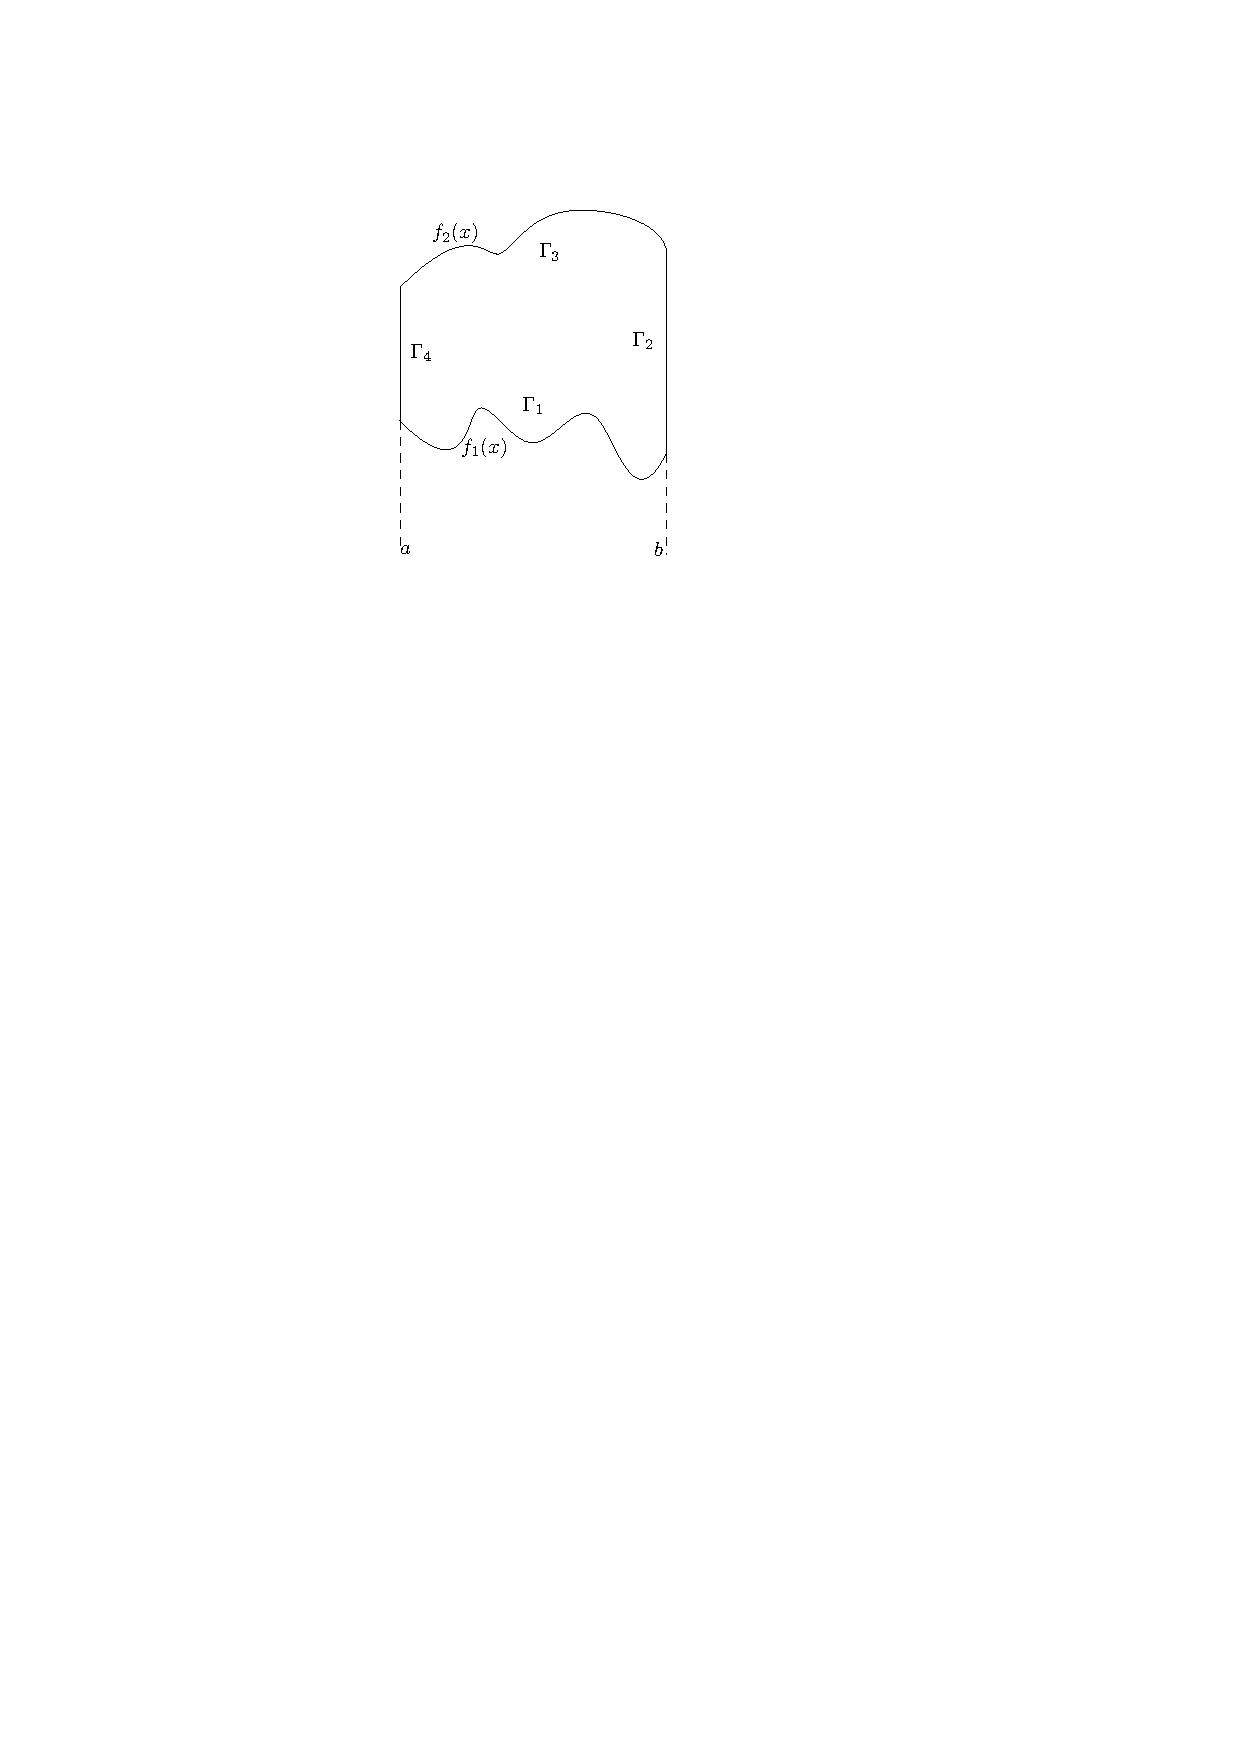
\includegraphics[scale=1.2]{dg/greenytype}
  \end{minipage} \hfill
  \begin{minipage}{0.68\linewidth}
    Тогда 
    $\displaystyle
    \int_\Gamma \omega = \int_{\Gamma_1} \omega + \int_{\Gamma_3} \omega =
      \int_a^b P(t,f_1(t)) - P(t,f_2(t))\, \del t
    $
    
    Тем временем, от $\displaystyle \iint_D \cdots$ осталось лишь 
    $(-1 )\cdot\dint_a^b\, \del x \; \int_{f_1(x)}^{f_2(x)} \pder{P}{y} \, \del y$.

    Как видно, получилось.
  \end{minipage}
  \vspace{1em}
  
  Произвольная область легко \note{нет} режется на области типа $y$. Склеивать их можно, так
  как интеграл по вертикальным сторонам 0.
  
  А потом сложить это с областями типа $x$.
\end{tproof}

\paragraph{Классическая формула Стокса}
\label{par:dg::stocks}

\begin{thrm}\label{thrm:dg::stocks}
  Пусть $M$~--- компактная ориентируемая поверхность в $\R^3$ с краем, $F$~--- гладкое векторное
  поле.
  Тогда
  \[
    \iint_M \langle \rot F , n\rangle \, \del S = \oint_{\partial M} \langle F,\tau \rangle\, \del s
  \]
\end{thrm}

\begin{tproof}
  Поскольку всё еще непонятно, что есть интеграл от формы по непростому многообразию, придётся
  ограничиться простыми.

  Пусть $F = (P,Q,R)$, $N=(A,B,C)$.
  Здесь можно снова занулить $Q, R$.
  Тогда \[
    \rot F n = \frac{1}{|N|} \Bigl\langle (0, P_z, -P_y) , N \Bigr\rangle 
    = \frac{1}{|N|} ( P_z B - P_y C )
  \]

  Тперь про вторую половину. \[
    \oint_\Gamma \langle F,\tau \rangle \, \del s 
    = \oint_{\ov~ \Gamma} P x_u \, \del u + Px_v \,\del v  
    =\oint_{\ov~ \Gamma} \ov~\omega 
  \]
  Здесь мы довольно коварно перешли от границы многообразия к границе пространства параметров.
  И ещё одна проблема как будто возникает из-за того, что в определении многообразия с границей
  граница вроде не замкнута. Да и вообще прямая. Впрочем, это лечится инверсией. А вот что
  делать бесконечностью~--- непонятно. Разве что сказать, что одна точка имеет меру ноль.
  
  Ладно, тут пользуемся  теоремой \ref{thrm:dg::green}, и получим первую половину.
\end{tproof}

\paragraph{Формула Гаусса-Остроградского}
\label{par:dg::gaussost}


\begin{thrm}\label{thrm:dg::gaussost}
  Пусть $V$~--- компактное тело в $\R^3$ с гладкой границей (гладким подмногообразием $\R^3$).
  Нормаль выберем <<наружу>>.  Тогда
  \[
    \oiint_M \langle F,n \rangle\, \del S = \iiint_V \div F\, \del V
  \]
\end{thrm}

\begin{tproof}
  Идейно мало чем отличается от теоремы Грина. 
  Тоже разбиваем всё на области с вертикальными гранями, а потом складываем.
\end{tproof}

Все равно все эти теоремы никому не нужны, а лучше пользоваться абстрактной формулой Стокса
\[
  \int_{\partial M} \omega  = \int_M \del \omega 
\]

\paragraph{Физический смысл дивергенции и ротора}
\label{par:dg::physdiv}

Дивергенция~--- удельный (по объему) поток через через бесконечно малую поверхность.
C ротором~--- сложно. Можно представить себе как-то так. Выделим контур (в жидкости)
и заморизим всё, кроме него. Тогда средняя скорость (усреднённая по площади!) будет
чем-то вроде ротора.

См Фейнмановские лекции по физике, том 5 или 6. Который про магнетизм.

\paragraph{Разные векторные поля}
\label{par:dg::vecftypes}

Попробуем в красивые таблички: \ref{tab:dg::vecftypes::prop}

\vspace{1em}

\begin{table}[h]
  \def\arraystretch{1.7}
  \caption{Разные поля}
  \vspace{0.5em}
  \label{tab:dg::vecftypes::prop}
  \begin{tabulary}{1.0\textwidth}{l c p{4em} L} \toprule
    \bf Название  & $F$            & $\omega_F$ & $\int \omega_F$  \\ \midrule
    Потенциальное & $F=\grad \Phi$ & точна, $p=1$ & ноль для любой петли. 
    Следует хоть из Ньютона-Лейбница.\\
    
    Безвихревое   & $\rot F = 0$ & замкнута, $p=1$  &
    ноль для петель, что граница какой-нибудь поверхности. 
    Можно проверить через формулу Стокса (\ref{thrm:dg::stocks}) \\
    
    Соленоидальное & $F = \rot B$ & точна, $p=2$ &
    $\displaystyle\iint_{M} \omega = 0$, $M$~--- замкнута.
    Проверяется тоже через Стокса, но в другую сторону.\\

    Безвихревое & $\div F = 0$ & замкнута, $p=2$ & ноль, для поверхностей, 
    являющихся краем трехмерных многообразий. Проверяется через Гаусса-Остроградского.
    (\ref{thrm:dg::gaussost})
    
    \\ \bottomrule
  \end{tabulary}
\end{table}

Из нечетных условий следуют чётные.
Наоборот работает лишь там, где любая петля стягивается в точку.


\paragraph{Примеры полей с разными свойствами}
\label{par:dg::vecfitwo}

вот тут уже точно по методичке Лодкина.



\end{document}
% vim: tw=100 cc=100

